% !TeX encoding = UTF-8
% !TeX spellcheck = ru_RU
% !TeX root = lecture1.tex

\documentclass[9pt]{beamer}

\usepackage{polyglossia}   %% загружает пакет многоязыковой вёрстки

\setmainlanguage{russian}  %% устанавливает главный язык документа
\setmainfont{Times New Roman}
\setromanfont{Times New Roman} 
\setmonofont{Fira Code} 
\setsansfont{Arial} 

\PolyglossiaSetup{russian}{indentfirst=true}

\newfontfamily{\cyrillicfont}{Times New Roman}[Ligatures=TeX]
\newfontfamily{\cyrillicfontrm}{Times New Roman}[Ligatures=TeX]
\newfontfamily{\cyrillicfonttt}{Fira Code}[Ligatures=TeX]
\newfontfamily{\cyrillicfontsf}{Arial}[Ligatures=TeX]

\usepackage{wasysym,amssymb}

\usepackage{pgfplots}
\usetikzlibrary{arrows,positioning,shapes}

\usepackage{minted}
\newminted{cpp}{frame=leftline,framerule=1.5pt,framesep=1em,breaklines=true,autogobble=true}

\usetheme{default}
\usecolortheme{seagull}
\useoutertheme[subsection=false]{miniframes}
\setbeamertemplate{mini frames}[tick]


\usepackage{ragged2e}

\usepackage{xcolor}

\makeatletter
\setbeamertemplate{section in head/foot}{%
    \parbox[c][0.33cm][t]{\dimexpr(\textwidth-1.3cm)/\beamer@sectionmax\relax}{%\
        \hyphenpenalty=9999\RaggedRight\fontsize{4}{4}\selectfont\insertsectionhead}}
\makeatother

\author{Воронин Андрей Андреевич}
\title{Лекция 1 – введение в язык C++}
\institute{Кафедра прикладной математики и информатики}
\date{\today}
\begin{document}
\titlepage 

\section{История языка C++}
\begin{frame}{Язык C}
    \begin{itemize}
        \item Язык программирования C разработан в начале 1973 года в
        компании Bell Labs Кеном Томпсоном и Деннисом Ритчи.
        \item Язык C был создан для использования в операционной
        системе UNIX.
        \item В связи с успехом UNIX язык C получил широкое
        распространение.
        \item На данный момент C является одним из самых
        распространенных языков программирования (доступен на
        большинстве платформ).
        \item C – основной язык низкоуровневой разработки.
        \item Язык программирования C++ создан на основе языка C.
    \end{itemize}
\end{frame}
\begin{frame}{Особенности языка C}
    \begin{itemize}
        \item \textbf{Эффективность.}\\
        Язык C позволяет писать программы, которые напрямую
        работают с железом.
        \item \textbf{Стандартизированность.}\\
        Спецификация языка C является международным
        стандартом.
        \item \textbf{Относительная простота.}\\
        Стандарт языка C занимает 520 страниц (Java 772, C++ 1605).
    \end{itemize}
\end{frame}
\begin{frame}{Создание C++}
    \begin{itemize}
        \item Разрабатывается с начала 1980-х годов.
        \item Создатель – сотрудник Bell Labs Бьёрн Страуструп.
        \item Изначально это было расширение языка C для поддержки
        работы с классами и объектами.
        \item Это позволило проектировать программы на более высоком
        уровне абстракции.
        \item Ранние версии языка назывались ”C with classes”.
        \item Первый компилятор cfront, перерабатывал исходный код ”C
        with classes” в исходный код на C.
    \end{itemize}
\end{frame}
\begin{frame}{Развитие C++}
    \begin{itemize}
        \item К 1983 году в язык были добавлены множество новых
        возможностей (виртуальные функции, перегрузка функций
        и операторов, ссылки, константы, ...)
        \item Получившийся язык перестал быть просто дополненной
        версией классического C и был переименован из ”C with
        classes” в C++.
        \item Имя языка, получившегося в итоге, происходит от оператора
        унарного постфиксного инкремента C ’++’ (увеличение
        значения переменной на единицу).
        \item Язык также не был назван D, поскольку ”является
        расширением C и не пытается устранять проблемы путем
        удаления элементов C”.
        \item Язык начинает активно развиваться. Появляются новые
        компиляторы и среды разработки.
    \end{itemize}
\end{frame}
\begin{frame}{Стандартизация C++}
    \begin{itemize}
        \item Лишь в 1998 году был ратифицирован международный
        стандарт языка C++: ISO/IEC 14882:1998 ”Standard for the
        C++ Programming Language”.
        \item В 2003 году был опубликован стандарт языка ISO/IEC
        14882:2003, где были исправлены выявленные ошибки и
        недочеты предыдущей версии стандарта.
        \item В 2005 году был выпущен Library Technical Report 1 (TR1).
        \item С 2005 года началась работа над новой версией стандарта,
        которая получила кодовое название C++0x.
        \item В конце концов в 2011 году стандарт был принят и получил
        название C++11 ISO/IEC 14882:2011.
        \item C++14 ISO/IEC 14882:2014 небольшое расширение и
        исправление ошибок предыдущего стандарта.
        \item Стандарт C++17 ISO/IEC 14882:2017 принес изменения
        направленные на большую безопасность языка.
        \item C++20 находится в разработке и обещает серьёзный набор
        изменений включающих изменение процесса сборки.
    \end{itemize}
\end{frame}
\begin{frame}{Совместимость C и C++}
    \begin{itemize}
        \item Один из принципов разработки стандарта C++ – это
        сохранение совместимости с C.
        \item Синтаксис C++ унаследован от языка C.
        \item C++ в строгом смысле не является надмножеством C.
        \item Можно писать программы на C так, чтобы они успешно
        компилировались на C++.
        \item C и C++ сильно отличаются как по сложности, так и по принятым архитектурным решениям, которые используются
        в обоих языках.
    \end{itemize}    
\end{frame}


\section{Характеристики языка C++}
\begin{frame}{Сложность C++}
    \textit{C makes it easy to shoot yourself in the foot. C++ makes it harder,
    but when you do, it blows away your whole leg.\\
    (В языке С легко прострелить себе ногу. В С++ это сложнее, но
    если вы сделаете это, то отстрелите всю ногу целиком.)}
    \begin{flushright}
        \textbf{Bjarne Stroustrup}
    \end{flushright}
    \vspace{2em}
    
   \textit{ Every extension proposal should be required to be accompanied by
    a kidney. People would submit only serious proposals, and nobody
    would submit more than two.\\
    (Нужно, чтобы к каждому предложению о расширении языка
    обязательно прилагалась почка. Тогда люди присылали бы
    только очень важные предложения, и никто не прислал бы
    более двух.)}
    \begin{flushright}
        \textbf{Jim Waldo}
    \end{flushright}
\end{frame}
\begin{frame}{Сложность C++}
    \begin{itemize}
        \item Описание стандарта занимает 1605 страниц текста.
        \item Нет никакой возможности рассказать ”весь C++” в рамках
        одного, путь даже очень большого курса.
        \item В C++ программисту позволено делать очень многое, и это
        влечет за собой большую ответственность.
        \item На плечи программиста ложится много дополнительной
        работы:
        \begin{itemize}
            \item проверка корректности данных,
            \item управление памятью,
            \item обработка низкоуровневых ошибок.
        \end{itemize}        
    \end{itemize}
\end{frame}
\begin{frame}{Мультипарадигменность}
    На языке C++ можно писать программы в рамках нескольких
    парадигм программирования:
    \begin{itemize}
        \item процедурное программирование
        (код ”в стиле C”);
        \item объектно-ориентированное программирование
        (классы, наследование, виртуальные функции, ...);
        \item обобщенное программирование
        (шаблоны функций и классов);
        \item функциональное программирование
        (функторы, безымянные функции, замыкания);
        \item генеративное программирование
        (метапрограммирование на шаблонах).
    \end{itemize}    
\end{frame}
\begin{frame}{Эффективность}
    Одна из фундаментальных идей языков C и C++ – отсутствие
    неявных накладных расходов, которые присутствуют в других
    более высокоуровневых языках программирования.
    \begin{itemize}
        \item Программист сам выбирает уровень абстракции, на котором
        писать каждую отдельную часть программы.
        \item Можно реализовывать критические по производительности
        участки программы максимально эффективно.
        \item Эффективность делает C++ основным языком для
        разработки приложений с компьютерной графикой (к
        примеру, игры).
    \end{itemize}
\end{frame}
\begin{frame}{Низкоуровневость}
    Язык C++, как и C, позволяет работать напрямую с ресурсами
    компьютера.
    \begin{itemize}
        \item Позволяет писать низкоуровневые системные приложения
        (например драйверы операционной системы).
        \item Неаккуратное обращение с системными ресурсами может
        привести к падению программы.
    \end{itemize}
    
    В C++ отсутствует автоматическое управление памятью.
    \begin{itemize}
        \item Позволяет программисту получить полный контроль над
        программой.
        \item Необходимость заботиться об освобождении памяти.
    \end{itemize}
\end{frame}
\begin{frame}{Компилируемость}
    C++ является компилируемым языком программирования.
    Для того, чтобы запустить программу на C++, ее нужно сначала
    \emph{скомпилировать}.
    Компиляция – преобразование текста программы на языке
    программирования в машинный код.
    \begin{itemize}
        \item Нет накладных расходов при исполнении программы.
        \item При компиляции можно отловить некоторые ошибки.
        \item Требуется компилировать для каждой платформы отдельно.
    \end{itemize}
\end{frame}
\begin{frame}{Статическая типизация}
    C++ является статически типизированным языком.
    \begin{enumerate}
        \item Каждая сущность в программе (переменная, функция и пр.)
        имеет свой тип,
        \item и этот тип определяется на момент компиляции.
    \end{enumerate}
    Это нужно для того чтобы
    \begin{enumerate}
        \item  вычислить размер памяти, который будет занимать каждая
        переменная в программе,
        \item  определить, какая функция будет вызываться в каждом
        конкретном месте.
    \end{enumerate}
    Всё это определяется на момент компиляции и "зашивается" в
    скомпилированную программу. В машинном коде никаких типов
    уже нет, там идет работа с последовательностями байтов.
\end{frame}
\begin{frame}
    Выберите все верные утверждения из списка.
    \begin{description}
        \item[\Square]  C++ ориентирован на написание эффективных
        приложений.
        \item[\Square]  C++ поддерживает объектно-ориентированное
        программирование.
        \item[\Square]  C++ не поддерживает процедурное
        программирование.
        \item[\Square]  C++ поддерживает процедурное
        программирование.
        \item[\Square]  C++ интерпретируемый язык программирования
        \item[\Square]  C++ ориентирован на безопасность работы с памятью.
    \end{description}
\end{frame}
\begin{frame}
    Выберите все верные утверждения из списка.
    \begin{description}
        \item[\XBox]  C++ ориентирован на написание эффективных
        приложений.
        \item[\XBox]  C++ поддерживает объектно-ориентированное
        программирование.
        \item[\Square]  C++ не поддерживает процедурное
        программирование.
        \item[\XBox]  C++ поддерживает процедурное
        программирование.
        \item[\Square]  C++ интерпретируемый язык программирования
        \item[\Square]  C++ ориентирован на безопасность работы с памятью.
    \end{description}
\end{frame}



\section{Зачем нужен компилятор?}
\begin{frame}{Что такое компиляция?}
    \begin{figure}
        \begin{tikzpicture}[every text node part/.style={align=center}]
            \node[inner sep=0pt] (Bjarnie) at (0,0)
            {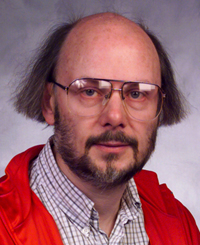
\includegraphics[width=.2\textwidth]{images/Stroustrup.jpg}};
            \node[draw,rectangle, right = 30mm of Bjarnie] (arch) {Архитектура \\ программы};
            \node[draw,rectangle, below = of arch] (code) {Код на C++};
            \node[draw,rectangle, below = of code] (mcode) {Машинный код};
            \node[inner sep=0pt, below right = 0mm and 10mm of mcode] (Fortnite)
            {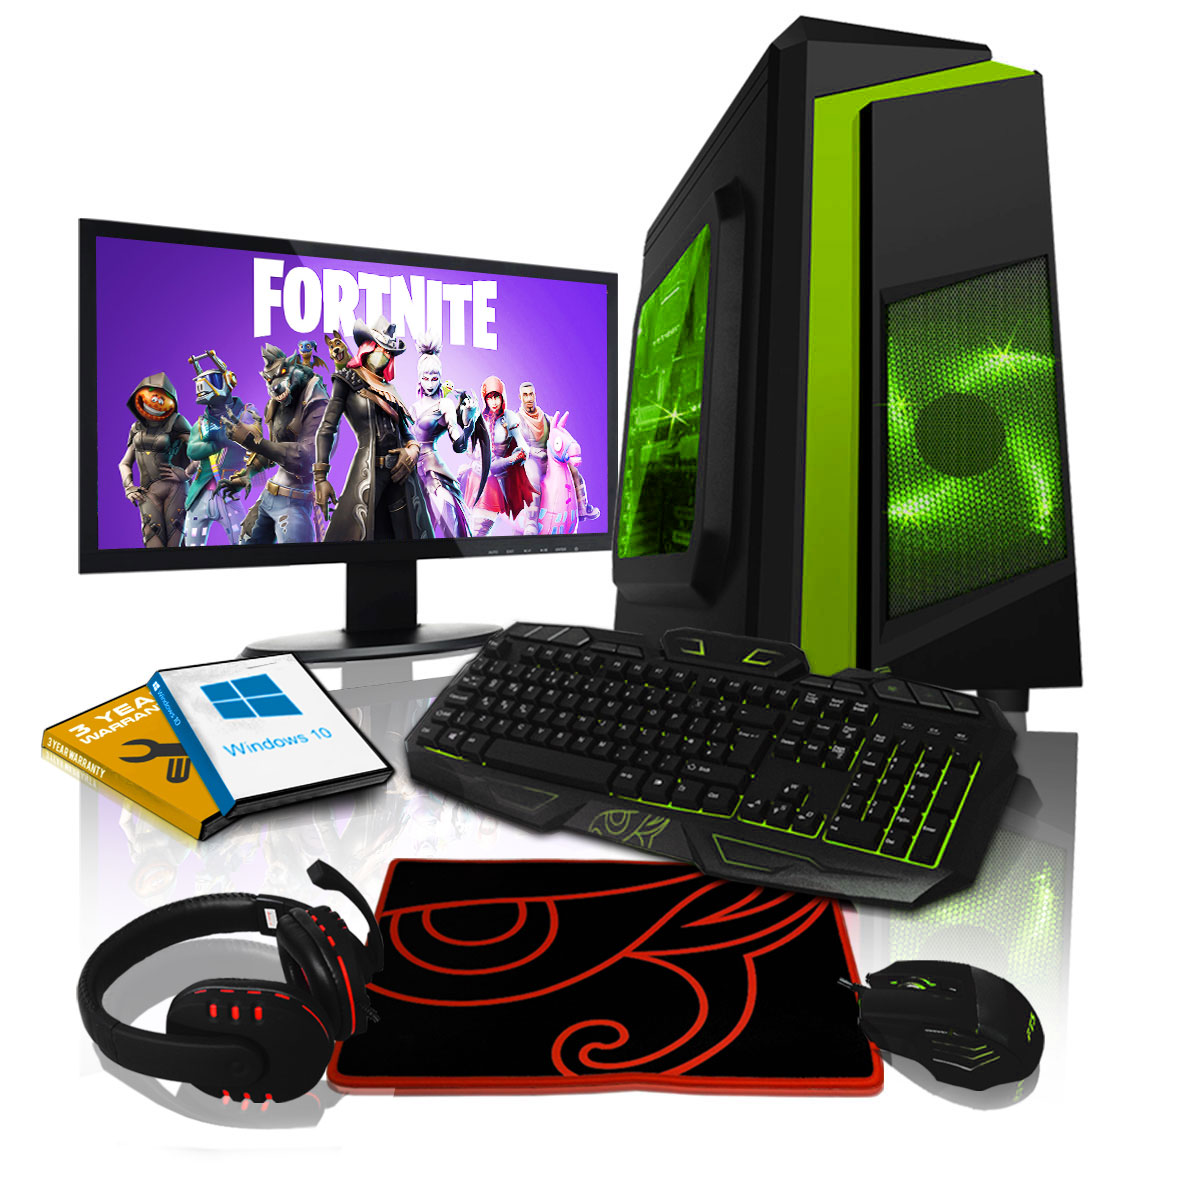
\includegraphics[width=.25\textwidth]{images/full-Fortnite-green-package.jpg}};
            
            \path[draw,-latex'](Bjarnie) -- node [text width=2.5cm,midway,above] {Проектирование} (arch);
            \path[draw,-latex'](arch) -- node [midway,right] {Программирование} (code);
            \path[draw,-latex'](code) -- node [midway,right] {Компиляция} (mcode);
            \path[draw,-latex'](mcode) |- node [midway,above right] {Исполнение} (Fortnite);
        \end{tikzpicture}
    \end{figure}
\end{frame}

\begin{frame}{Что такое компиляция?}
    \begin{figure}
        \begin{tikzpicture}[every text node part/.style={align=center}]
        \node[inner sep=0pt] (James) at (0,0)
        {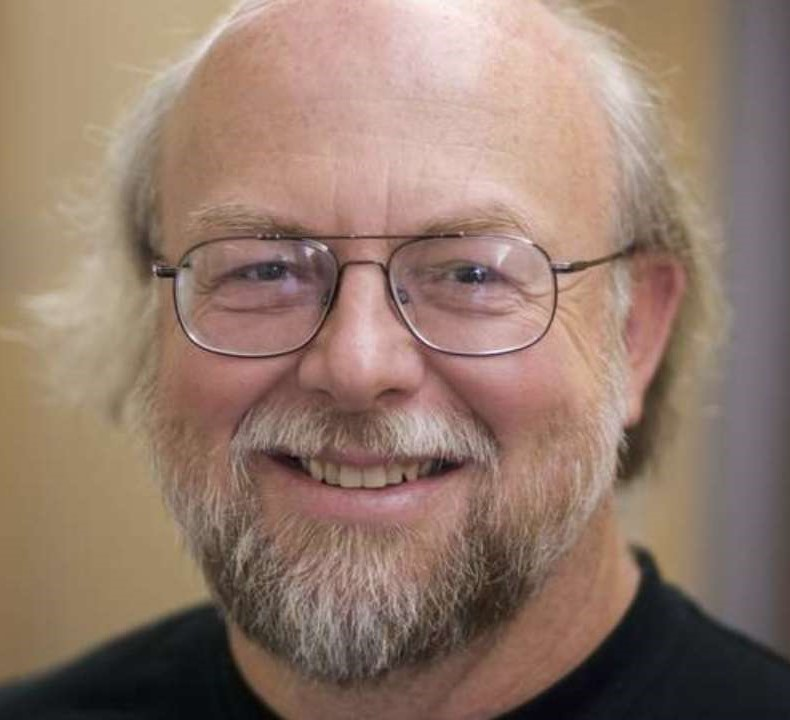
\includegraphics[width=.2\textwidth]{images/James-Gosling.jpg}};
        \node[draw,rectangle, right = 30mm of James] (arch) {Архитектура \\ программы};
        \node[draw,rectangle, below = of arch] (code) {Код на Java};
        \node[draw,rectangle, below = of code] (bcode) {Байт код};
        \node[draw,circle, left = 30mm of bcode] (JVM) {Java Virtual \\ Machine (JVM)};
        \node[inner sep=0pt, below right = 5mm and -3mm of mcode] (eclipse)
        {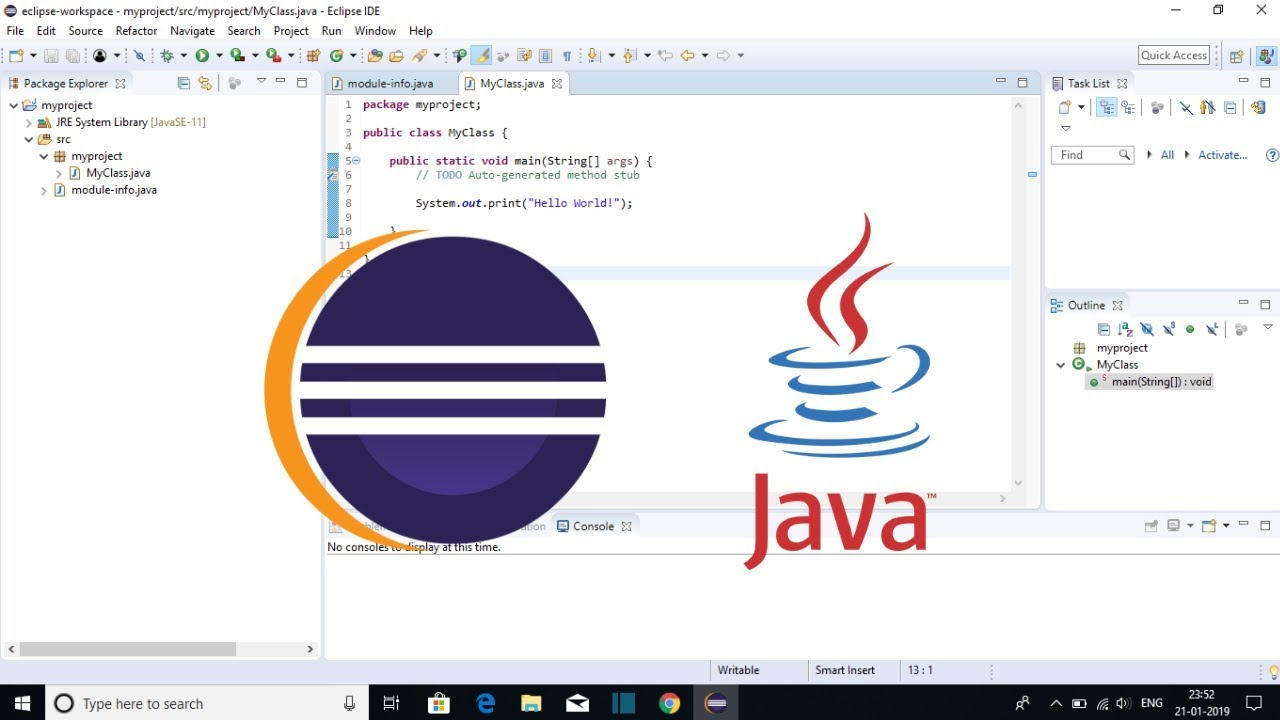
\includegraphics[width=.40\textwidth]{images/eclipse.jpg}};
        
        \path[draw,-latex'](James) -- node [text width=2.5cm,midway,above ] {Проектирование} (arch);
        \path[draw,-latex'](arch) -- node [midway,right] {Программирование} (code);
        \path[draw,-latex'](code) -- node [midway,right] {Компиляция} (bcode);
        \path[draw,-latex'](bcode) -- node [midway,above] {Исполнение} (JVM);
        \path[draw,latex'-latex'](JVM) |- node [near end,above right] {Трансляция команд} (eclipse);
        \end{tikzpicture}
    \end{figure}
\end{frame}


\begin{frame}{Что такое компиляция?}
    \begin{figure}
        \begin{tikzpicture}[every text node part/.style={align=center}]
        \node[inner sep=0pt] (Larry) at (0,0)
        {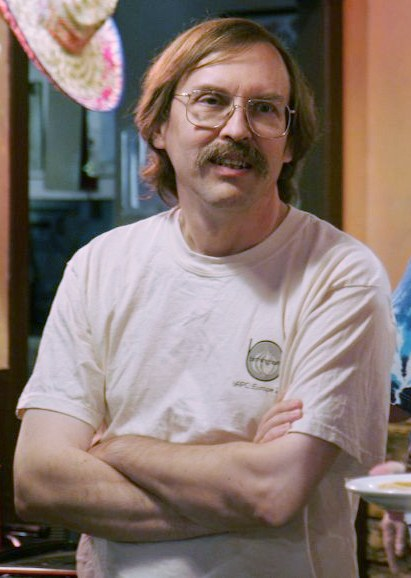
\includegraphics[width=.2\textwidth]{images/Larry_Wall_YAPC_2007.jpg}};
        \node[draw,rectangle, right = 30mm of Larry] (arch) {Архитектура \\ программы};
        \node[draw,rectangle, below = of arch] (code) {Код на Perl};
        \node[draw,inner sep=-5pt,regular polygon,regular polygon sides=7, below left = 3 mm and 30mm of code] (Perl) {Perl \\ интерпретатор};
        \node[inner sep=0pt, below right = 15mm and 0mm of code] (perllogo)
        {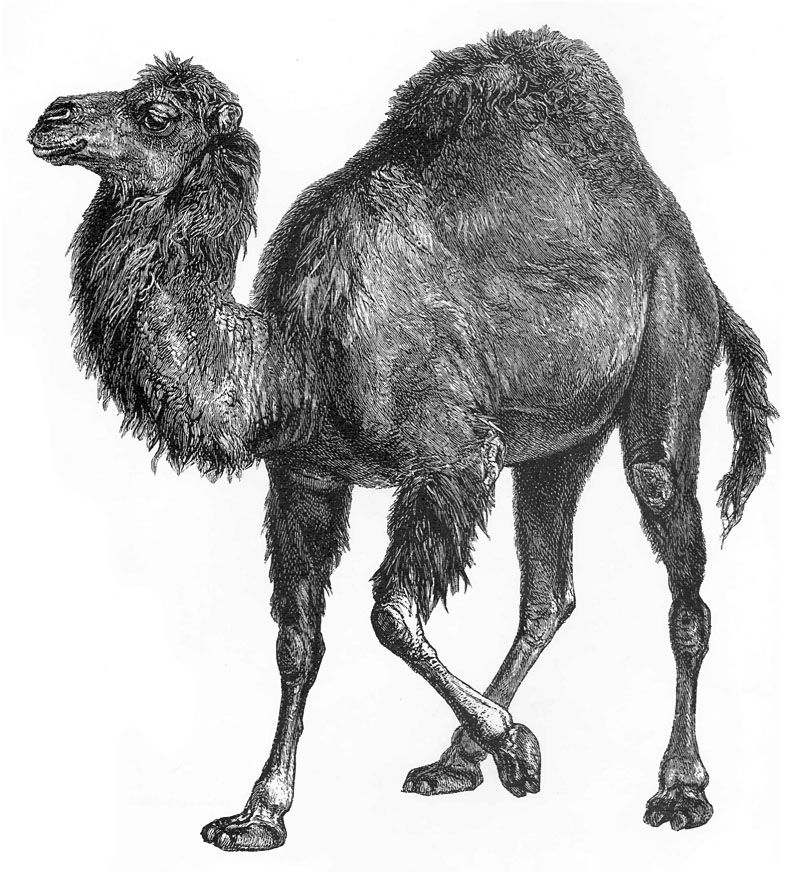
\includegraphics[width=.25\textwidth]{images/perl.jpg}};
        
        \path[draw,-latex'](Larry) -- node [text width=2.5cm,midway,above ] {Проектирование} (arch);
        \path[draw,-latex'](arch) -- node [midway,right] {Программирование} (code);
        \path[draw,-latex'](code) |- node [midway,above left] {Интерпретация} (Perl);

        \path[draw,latex'-latex'](Perl) |- node [near end,above right] {Трансляция команд} (perllogo);
        \end{tikzpicture}
    \end{figure}
\end{frame}

\begin{frame}{Плюсы и минусы компилируемости в машинный код}
    \textbf{Плюсы}
    \begin{itemize}
        \item эффективность: программа компилируется и оптимизируется для конкретного процессора
        \item нет необходимости устанавливать сторонние приложения (такие как интерпретатор или виртуальная машина).
    \end{itemize}
    \textbf{Минусы}
    \begin{itemize}
        \item нужно компилировать для каждой платформы
        \item сложность внесения изменений в программу -- нужно перекомпилировать заново.
    \end{itemize}
    \textbf{Важно}: компиляция -- преобразование одностороннее, нельзя восстановить исходный код.
\end{frame}

\begin{frame}
    Выберите все верные утверждения из списка.
    \begin{description}
        \item[\Square]  Код программы, написанный на интерпретируемом языке, можно без предварительной компиляции запустить на любой платформе, где есть интерпретатор этого языка.
        \item[\Square]  Код программы, написанный на языке, который компилируется в байт код виртуальной машины, достаточно скомпилировать однажды, чтобы программу можно было запускать на любой платформе, где есть соответствующая виртуальная машина.
        \item[\Square]  Для запуска программы, код которой был написан на компилируемом языке, на компьютере должен быть установлен компилятор этого языка.
        \item[\Square]  Код программы, написанный на языке, который компилируется в машинный код, достаточно скомпилировать однажды, и потом программу можно будет запустить на любой платформе.
        \item[\Square] Для запуска программы, код которой был написан на интерпретируемом языке, на компьютере должен быть установлен интерпретатор этого языка.
        \item[\Square] Скомпилировать программу на C++ для некоторой архитектуры X можно только на компьютере с архитектурой X.
    \end{description}
\end{frame}

\begin{frame}
    Выберите все верные утверждения из списка.
    \begin{description}
        \item[\XBox]  Код программы, написанный на интерпретируемом языке, можно без предварительной компиляции запустить на любой платформе, где есть интерпретатор этого языка.
        \item[\XBox]  Код программы, написанный на языке, который компилируется в байт код виртуальной машины, достаточно скомпилировать однажды, чтобы программу можно было запускать на любой платформе, где есть соответствующая виртуальная машина.
        \item[\Square]  Для запуска программы, код которой был написан на компилируемом языке, на компьютере должен быть установлен компилятор этого языка.
        \item[\Square]  Код программы, написанный на языке, который компилируется в машинный код, достаточно скомпилировать однажды, и потом программу можно будет запустить на любой платформе.
        \item[\XBox] Для запуска программы, код которой был написан на интерпретируемом языке, на компьютере должен быть установлен интерпретатор этого языка.
        \item[\Square] Скомпилировать программу на C++ для некоторой архитектуры X можно только на компьютере с архитектурой X.
    \end{description}
\end{frame}

\section{Структура кода на C++}
\begin{frame}{Разбиение программы на файлы}
    Зачем разбивать программу на файлы?
    \begin{itemize}
        \item С небольшими файлами удобнее работать.
        \item Разбиение на файлы структурирует код.
        \item Позволяет нескольким программистам разрабатывать приложение одновременно.
        \item Ускорение повторной компиляции при небольших изменениях в отдельных частях программы.
    \end{itemize}
    Файлы с кодом на C++ бывают двух типов:
    \begin{enumerate}
        \item файлы с исходным кодом (расширение \texttt{.cpp}, \texttt{.cxx}, \texttt{.cc} иногда \texttt{.C})
        \item заголовочные файлы (расширение \texttt{.hpp}, \texttt{hxx}, \texttt{hh}  или \texttt{.h})
    \end{enumerate}
\end{frame}


\begin{frame}[fragile]{Заголовочные файлы}
    \framesubtitle{Определение функции}
    Файл \texttt{foo.cpp}:
    \begin{cppcode}
        // определение (defenition) функции foo
        void foo()
        {
            bar();        
        }
    \end{cppcode}
        
    \vspace{2em}
    Файл \texttt{bar.cpp}:
    \begin{cppcode}
        // определение (defenition) функции bar
        void bar(){ }
    \end{cppcode}
    
    \vspace{2em}
    Компиляция этих файлов вызовет ошибку.
\end{frame}

\begin{frame}[fragile]{Заголовочные файлы}
\framesubtitle{Объявление  и определение}
    Файл \texttt{foo.cpp}:
    \begin{cppcode}
        // объявление (declaration) функции bar
        void bar();
        
        // определение (defenition) функции foo
        void foo()
        {
            bar();        
        }
    \end{cppcode}

    \vspace{2em}
    Файл \texttt{bar.cpp}:
    \begin{cppcode}
        // определение (defenition) функции bar
        void bar(){ }
    \end{cppcode}
\end{frame}


\begin{frame}[fragile]{Заголовочные файлы}
\framesubtitle{Неопределенное поведение}
    Файл \texttt{foo.cpp}:
    \begin{cppcode}
        void bar();
        
        void foo()
        {
            bar();        
        }
    \end{cppcode}

    \vspace{2em}
    Файл \texttt{bar.cpp}:
    \begin{cppcode}
        // определение (defenition) функции bar
        int bar(){ return 1; }
    \end{cppcode}

    \vspace{2em}
    Данный код некорректен -- объявление отличается от определения. (Неопределенное поведение.)
\end{frame}


\begin{frame}[fragile]{Заголовочные файлы}
    \framesubtitle{Подключение заголовочных файлов}
    Файл \texttt{foo.cpp}:
    \begin{cppcode}
        #include "bar.hpp"
        
        void foo()
        {
            bar();        
        }
    \end{cppcode}
    
    \vspace{2em}
    Файл \texttt{bar.cpp}:
    \begin{cppcode}
        int bar(){ return 1; }
    \end{cppcode}

    \vspace{2em}
    Файл \texttt{bar.hpp}:
    \begin{cppcode}
        int bar();
    \end{cppcode}    
\end{frame}


\begin{frame}[fragile]{Заголовочные файлы}
    \framesubtitle{Двойное включение}
    Может случиться двойное включение заголовочного файла.
    Файл \texttt{foo.cpp}:
    \begin{cppcode}
        #include "foo.hpp"
        #include "bar.hpp"
        
        void foo()
        {
            bar();        
        }
    \end{cppcode}
    
    \vspace{2em}
    Файл \texttt{foo.hpp}:
    \begin{cppcode}
        #include "bar.hpp"
        
        int foo();
    \end{cppcode}  
\end{frame}


\begin{frame}[fragile]{Заголовочные файлы}
    \framesubtitle{Защита от двойного включения}
    Предыдущую ситуацию можно исправить двумя способами:
    \begin{itemize}
    \item (наиболее переносимо) Файл \texttt{bar.hpp}:
    \begin{cppcode}
        #ifndef BAR_HPP
        #define BAR_HPP
        
        int bar();
        
        #endif //BAR_HPP
    \end{cppcode}

    \item (наиболее просто) Файл \texttt{bar.hpp}:
    \begin{cppcode}
        #pragma once
        
        int bar();
    \end{cppcode}  
    \end{itemize}
    
\end{frame}

\begin{frame}[fragile]{Объявление и определение}
    \textbf{Объявление (declaration)} — вводит имя, возможно, не определяя деталей. Например, ниже перечислены объявления:
    \begin{itemize}
        \item \mintinline{cpp}{int a;}
        \item \mintinline{cpp}{void foo();}
        \item \mintinline{cpp}{void bar() { foo(); }}
    \end{itemize}

    \textbf{Определение (definition)} — это объявление, дополнительно определяющее детали, необходимые компилятору. Из перечисленных выше объявлений, определениями являются только два:
    \begin{itemize}
        \item \mintinline{cpp}{int a;}
        \item \mintinline{cpp}{void bar() { foo(); }}
    \end{itemize}

    Для определения переменной достаточно указать ее тип, а для определения функций, кроме имени, типов параметров и возвращаемого значения, нужно указать еще тело функции. Проще говоря, определение содержит всю информацию, необходимую компилятору, чтобы выделить память для хранения объекта.
    
    В C++ есть также возможность объявить переменную, не определяя ее: \\
    \mintinline{cpp}{extern int a;}
\end{frame}

\begin{frame}[fragile]{Объявление и определение}
    \begin{itemize}
        \item \mintinline{cpp}{extern int a;} -- объявление переменной типа \texttt{int},
        \item \mintinline{cpp}{int a;} -- объявление и \textbf{определение} переменной типа \texttt{int},
        \item \mintinline{cpp}{void foo();} -- объявление функции с именем \texttt{foo}
        \item \mintinline{cpp}{void bar(){ foo(); }} -- объявление и \textbf{определение} функции с именем \texttt{bar}
    \end{itemize}
\end{frame}

\begin{frame}
    Интересно отметить, что файлы стандартной библиотеки C++ не используют расширение вовсе, например:
    \begin{itemize}
        \item iostream,
        \item algorithm,
        \item vector.
    \end{itemize}
    Разделение на файлы с исходным кодом и заголовочные файлы чисто условное, нет правил, запрещающих использовать .cpp файл как заголовочный, однако мы не рекомендуем так делать — использование общепринятых правил именования файлов упростит жизнь вам и вашим коллегам.
    
    Не стоит помещать \emph{определения} в заголовочные файлы без явной необходимости. В C++ есть способы, позволяющие поместить определение в заголовочный файл, не вызвав при этом ошибки компоновщика, но, как правило, это приводит к увеличению объектного файла и программы в целом
\end{frame}

\begin{frame}
    Выберите из списка объявления, которые \textbf{не} стоит помещать в заголовочные файлы.
    \begin{description}[align=left]
        \item[\Square] \mintinline{cpp}{void foo() { std::cout << "Hello, World!\n"; }}
        \item[\Square] \mintinline{cpp}{void foo();}
        \item[\Square] \mintinline{cpp}{int a;}
        \item[\Square] \mintinline{cpp}{extern int a;}
        \item[\Square] \mintinline{cpp}{void bar() { foo(); }}
    \end{description}
\end{frame}

\begin{frame}
    Выберите из списка объявления, которые \textbf{не} стоит помещать в заголовочные файлы.
    \begin{description}[align=left]
        \item[\XBox] \mintinline{cpp}{void foo() { std::cout << "Hello, World!\n"; }}
        \item[\Square] \mintinline{cpp}{void foo();}
        \item[\XBox] \mintinline{cpp}{int a;}
        \item[\Square] \mintinline{cpp}{extern int a;}
        \item[\XBox] \mintinline{cpp}{void bar() { foo(); }}
    \end{description}
\end{frame}

\section{Как компилируется программа на C++}
\begin{frame}[fragile]{Этап №1: Препроцессор}
    \begin{itemize}
        \item Язык препроцессора -- это специальный язык программирования, встроенный в C++.
        \item Препроцессор работает с кодом на C++ как с текстом.
        \item Команды языка препроцессора называют директивами, все директивы начинаются со знака \mintinline{cpp}{#}.
        \item Директива \mintinline{cpp}{#include} позволяет подключать заголовочные файлы к файлам кода.
        \begin{enumerate}
            \item \mintinline{cpp}{#include <foo.h>} -- библиотечный заголовочный файл,
            \item \mintinline{cpp}{#include "bar.h"} -- локальный заголовочный файл.
        \end{enumerate}
        \item Препроцессор заменяет директиву \mintinline{cpp}{#include "bar.h"} на содержимое файла \texttt{bar.h}.
    \end{itemize}
\end{frame}

\begin{frame}{Этап №2: Компиляция}
    \begin{itemize}
        \item На вход компилятору поступает код на C++ после обработки препроцессором.
        \item Каждый файл с кодом компилируется отдельно и независимо от других файлов с кодом.
        \item Компилируются только файлы с кодом (т.е. \texttt{*.cpp}).
        \item Заголовочные файлы сами по себе ни во что не компилируются, только в составе файлов с кодом.
        \item На выходе компилятора из каждого файла с кодом получается "объектный файл" -- бинарный файл со скомпилированным кодом (с расширением \texttt{.o} или \texttt{.obj}).
    \end{itemize}
\end{frame}

\begin{frame}[fragile]{Этап №3: Линковка (компоновка)}
    \begin{itemize}
        \item На этом этапе все объектные файлы объединяются в один исполняемый (или библиотечный) файл.
        \item Пр этом происходит подстановка адресов функций в места их вызова.
        \begin{cppcode}
            void foo()
            {
                bar();
            }
        \end{cppcode}
        
        \vspace{1em}
        \begin{cppcode}
            void bar() { }
        \end{cppcode}
        \item По каждому объектному файлу строится таблица всех функций, которые в нем определены.
    \end{itemize}
\end{frame}

\begin{frame}[fragile]{Этап №3: Линковка (компоновка)}
    \begin{itemize}
        \item На этапе компоновки важно, что каждая функция имеет уникальное имя.
        \item В C++ может быть две функции с одним именем, но разными параметрами. 
        \item Имена функций искажаются (mangle) таким образом, что в их имени кодируются их параметры.\\
        Например, компилятор GCC превратит имя функции \texttt{foo}
        
        \begin{cppcode}
            void foo(int a, double b) {}
        \end{cppcode}

    в \texttt{\_Z3fooid}
    \end{itemize}
\end{frame}


\begin{frame}[fragile]{Этап №3: Линковка (компоновка)}
    \begin{itemize}
        \item \emph{Точка входа} -- функция, вызываемая при запуске программы. По умолчанию -- это функция \texttt{main}:
        \begin{cppcode}
            int main()
            {
                return 0;
            }
        \end{cppcode}
        или
        \begin{cppcode}
            int main(int argc, char **argv)
            {
                return 0;
            }
        \end{cppcode}
    \end{itemize}
\end{frame}

\begin{frame}{Общая схема}
    \begin{figure}
        \begin{tikzpicture}[every text node part/.style={align=center}]
        \node[draw,rectangle,minimum height=1cm, minimum width = 2cm] (file1cpp) at (0,0) {\texttt{file1.cpp}};
        \node[draw,rectangle,minimum height=1cm, minimum width = 2cm] (file1o) at (5,0) {\texttt{file1.o}};
        \node[draw,rectangle,minimum height=1cm, minimum width = 2cm] (file2cpp) at (0,-2) {\texttt{file2.cpp}};
        \node[draw,rectangle,minimum height=1cm, minimum width = 2cm] (file2o) at (5,-2) {\texttt{file2.o}};
        
        \node[draw,rectangle,minimum height=1cm, minimum width = 2cm] (fileNcpp) at (0,-5) {\texttt{fileN.cpp}};
        \node[draw,rectangle,minimum height=1cm, minimum width = 2cm] (fileNo) at (5,-5) {\texttt{fileN.o}};
        
        \node[draw,rectangle,minimum height=1cm, minimum width = 2cm] (program) at (9,-2.5) {\texttt{program}};
        
        \path (file2cpp) -- node [midway] {\vdots} (fileNcpp);
        \path (file2o) -- node [midway] {\vdots} (fileNo);
        
        \path[draw,-latex'](file1cpp) -- node [text width=5cm,midway,above ] {Компиляция} (file1o);
        \path[draw,-latex'](file2cpp) -- (file2o);
        \path[draw,-latex'](fileNcpp) -- (fileNo);
        \path[draw,-latex'](file1o) -- node [midway,above right] {Линковка} (program);
        \path[draw,-latex'](file2o) -- (program);
        \path[draw,-latex'](fileNo) -- (program);
        \end{tikzpicture}
    \end{figure}
\end{frame}

\begin{frame}
    Выберите все верные утверждения из списка.
    \begin{description}[align=left]
        \item[\Square] Даже для программы состоящей из одной пустой функции \mintinline{cpp}{int main() { return 0; }} все равно требуется линковка.
        \item[\Square] Если в коде C++ вы вызываете необъявленную функцию, то это не ошибка, при условии, что функция была где-то определена.
        \item[\Square] Если в коде C++ вы вызываете функцию, которая была объявлена, но не была определена, то это ошибка этапа компиляции.
        \item[\Square] Для программы, состоящей всего из одного файла, не требуется линковка.
        \item[\Square] Если в коде C++ вы вызываете необъявленную функцию, то это ошибка этапа компиляции.
        \item[\Square] Если в коде C++ вы вызываете функцию, которая была объявлена, но не была определена, то это ошибка этапа линковки.
    \end{description}
\end{frame}


\begin{frame}
    Выберите все верные утверждения из списка.
    \begin{description}[align=left]
        \item[\XBox] Даже для программы состоящей из одной пустой функции \mintinline{cpp}{int main() { return 0; }} все равно требуется линковка.
        \item[\Square] Если в коде C++ вы вызываете необъявленную функцию, то это не ошибка, при условии, что функция была где-то определена.
        \item[\Square] Если в коде C++ вы вызываете функцию, которая была объявлена, но не была определена, то это ошибка этапа компиляции.
        \item[\Square] Для программы, состоящей всего из одного файла, не требуется линковка.
        \item[\XBox] Если в коде C++ вы вызываете необъявленную функцию, то это ошибка этапа компиляции.
        \item[\XBox] Если в коде C++ вы вызываете функцию, которая была объявлена, но не была определена, то это ошибка этапа линковки.
    \end{description}
\end{frame}

\section{Введение в синтаксис}
\begin{frame}{Типы данных}
    \begin{itemize}
        \item<1-> Целочисленные:
        \only<1>{
        \begin{enumerate}
            \item \mintinline{cpp}{char} 
            \item \mintinline{cpp}{short int}
            \item \mintinline{cpp}{int}
            \item \mintinline{cpp}{long int}
            \item \mintinline{cpp}{long long int}
        \end{enumerate}}
        \only<2->{
        \begin{enumerate}
            \item \mintinline{cpp}{int8_t} 
            \item \mintinline{cpp}{int16_t}
            \item \mintinline{cpp}{int32_t}
            \item \mintinline{cpp}{int32_t}
            \item \mintinline{cpp}{int64_t}
        \end{enumerate}}
        Могут быть беззнаковыми (\mintinline{cpp}{unsigned} или \mintinline{cpp}{uint8_t})
        \begin{itemize}
            \item $ -2^{n-1} \ldots (2^{n-1}-1) $ ($n$ -- число бит)
            \item $ 0 \ldots (2^{n}-1) $ (для \mintinline{cpp}{unsigned})
        \end{itemize}
        \item Числа с плавающей точкой:
        \begin{enumerate}
            \item \mintinline{cpp}{float}, 4 байта, 7 значащих цифр.
            \item \mintinline{cpp}{double}, 8 байт, 15 значащих цифр.
        \end{enumerate}
        \item Логический тип данных \mintinline{cpp}{bool}.
        \item Пустой тип \mintinline{cpp}{void}.        
    \end{itemize}
\end{frame}

\begin{frame}{Литералы}
    \begin{itemize}
        \item Целочисленные:
        \begin{enumerate}
            \item \mintinline{cpp}{'a'} -- код буквы \texttt{'a'}, тип \mintinline{cpp}{char}.
            \item \mintinline{cpp}{42} -- все целые по умолчанию типа \mintinline{cpp}{int}.
            \item \mintinline{cpp}{123456789L} -- суффикс \texttt{'L'} соответствует типу \mintinline{cpp}{long}.
            \item \mintinline{cpp}{1703U} -- суффикс \texttt{'U'} соответствует типу \mintinline{cpp}{unsigned int}.
            \item \mintinline{cpp}{1703UL} -- суффикс \texttt{'UL'} соответствует типу \mintinline{cpp}{unsigned long}.
        \end{enumerate}
        \item Числа с плавающей точкой:
        \begin{enumerate}
            \item \mintinline{cpp}{3.14} -- все числа с точкой по умолчанию \mintinline{cpp}{double}.
            \item \mintinline{cpp}{3.1415F} -- суффикс \texttt{'F'} соответствует типу \mintinline{cpp}{float}.
            \item \mintinline{cpp}{3.0E8} -- соответствует  $ 3\cdot10^8 $
        \end{enumerate}
        \item \mintinline{cpp}{true} \mintinline{cpp}{false} -- значения типа \mintinline{cpp}{bool}.
        \item Строки задаются в двойных кавычках: \mintinline{cpp}{"Test string"}.
    \end{itemize}
\end{frame}

\begin{frame}[fragile]{Переменные}
    \begin{itemize}
        \item При определении переменной указывается её тип. При определении можно сразу задать начальное значение (инициализация).
        \begin{cppcode}
            int i = 10;
            short j = 20;
            bool b = false;
            
            unsigned long l = 123321;
            
            double x = 13.5, y = 3.1415;
            float z;
        \end{cppcode}
    \item Нельзя оставлять переменные неинициализированными.
    \item Нельзя создать переменную пустого типа \mintinline{cpp}{void}.
    \end{itemize}
\end{frame}

\begin{frame}[fragile]{Операции}
    \begin{columns}
        \begin{column}{0.5\textwidth}
            \begin{itemize}
                \item Оператор присваивания: \alert{\texttt{=}}.
                \item Арифметические: 
                \begin{enumerate}
                    \item бинарные: \alert{\texttt{+ - * / \%}},
                    \item унарные: \alert{\texttt{++ --}}.
                \end{enumerate}
                \item Логические:
                \begin{enumerate}
                    \item бинарные: \alert{\texttt{\&\& ||}}
                    \item унарные: \alert{\texttt{!}}.
                \end{enumerate}
                \item Сравнения: \alert{\texttt{== != > < >= <=}}.
                \item Приведения типов: \alert{\texttt{(type)}}.
                \item Сокращенные версии бинарных операторов: \alert{\texttt{+= -= *= /= \%=}}.
            \end{itemize}
        \end{column}
        \begin{column}{0.5\textwidth}  %%<--- here
            \begin{cppcode}
                int i = 10;
                i = (20 * 3) % 7;
                
                int k = i++;
                int l = --i;
                
                bool b = !(k == 1);
                
                b = (a == 0) || (1 / a < 1);
                
                double d = 3.1415;
                float f = (int) d;
                
                // d = d * (i + k);
                d *= i + k;
            \end{cppcode}
        \end{column}
    \end{columns}
\end{frame}

\begin{frame}{Целочисленные типы в C++}
    Все целочисленные типы (кроме \texttt{char}) являются знаковыми. Беззнаковые версии типов определяется с ключевым словом \texttt{unsigned}, например: \texttt{unsigned short int}, \texttt{unsigned int} или \texttt{unsigned long int}. Для симметрии в языке предусмотрено явное указание того, что тип является знаковым — ключевое слово \texttt{signed} (используется редко).
    
    Более того, C++ допускает использование следующих сокращений:
    \begin{itemize}
        \item \texttt{unsigned} вместо \texttt{unsigned int},
        \item \texttt{short} вместо \texttt{short int},
        \item \texttt{long} вместо \texttt{long int}.
    \end{itemize}

    \textbf{Операции инкремента и декремента:}
\end{frame}

\begin{frame}[fragile]{Операции инкремента и декремента}
    \begin{cppcode}
        int a = 10; // a = 10
        int b = ++a; // префиксный инкремент возвращает новое значение => b = 11 и a = 11
        int c = a++; // постфиксный инкремент возвращает старое значение => с = 11 и a = 12
    \end{cppcode}
\end{frame}

\begin{frame}[fragile]{Преобразования типов в операторах}
    Выражениям так же как и значениям в C++ приписывается некоторые типы. Например, если \texttt{a} и \texttt{b} — это переменные типа \texttt{int}, то выражения \texttt{(a + b)}, \texttt{(a - b)}, \texttt{(a * b)} и \texttt{(a / b)} тоже будут иметь тип \texttt{int}.
    
    Важно всегда понимать, какой тип у выражения, которое вы написали в программе. Давайте проиллюстрируем это на следующем примере:
    
    \begin{cppcode}
        int a = 20;
        int b = 50;
        double d = a / b;  // d = 0, оба аргумента целочисленные, а значит деление целочисленное 
    \end{cppcode}

    Для того чтобы исправить эту ситуацию хотя бы один из аргументов оператора деления должен иметь типа double. Этого можно добиться при помощи уже известного нам оператора приведения типов:
    \begin{cppcode}
        double d = (double)a / b;  // d = 0.4
    \end{cppcode}

    Почему это сработало? Дело в том, что операторы для встроенных типов C++ \emph{всегда} работают с \emph{одинаковыми типами} аргументов. Если аргументы имеют разные типы, то происходит преобразование типов (promotion).
\end{frame}

\begin{frame}{Правило преобразования встроенных типов в операторах}
    Рассмотрим выражение \mintinline{cpp}{(a + b)}, где вместо \texttt{'+'} может стоять любой другой подходящий оператор.
    \begin{enumerate}
        \item Если один из аргументов имеет числовой тип с плавающей точкой, то второй аргумент приводится к этому типу (например, при сложении \texttt{double} и \texttt{int} значение типа \texttt{int} приводится к \texttt{double}).
        \item Если оба аргумента имеют числовой тип с плавающей точкой, то выбирается наибольший из этих типов (например, при сложении \texttt{double} и \texttt{float} значение типа \texttt{float} приводится к \texttt{double}).
        \item Если оба аргумента целочисленные, но их типы меньше \texttt{int}, то оба аргумента приводятся к типу \texttt{int} (например, при сложении двух значений типа \texttt{char} они оба сначала приводятся к \texttt{int}).
        \item Если оба аргумента целочисленные, то аргумент с меньшим типом приводится к типу второго аргумента (например, при сложении \texttt{long} и \texttt{int} значение типа \texttt{int} приводится к \texttt{long}).
        \item Если оба аргумента целочисленные и имеют тип одного размера, то предпочтение отдаётся беззнаковому типу (например, при сложении \texttt{int} и \texttt{unsigned int} значение типа \texttt{int} приводится к \texttt{unsigned int}).
    \end{enumerate}
\end{frame}

\begin{frame}[fragile]{Следствия неявных преобразований типов}
    \begin{enumerate}
        \item Следите за тем, какие типы участвуют в выражении, от этого может зависеть его значение.
        \item Не стоит использовать целочисленные типы меньше \texttt{int} в арифметических выражениях, они всё равно будут приведены к \texttt{int}.
        \item \alert{Не стоит смешивать \texttt{unsigned} и \texttt{signed}} типы в одном выражении, это может привести к неприятным последствиям.
    \end{enumerate}

    Для иллюстрации последнего следствия давайте рассмотрим следующий пример:
    \begin{cppcode}
        unsigned from = 100;
        unsigned to = 0;
        for (int i = from; i >= to; --i) {  ....  }
    \end{cppcode}    
\end{frame}

\begin{frame}[fragile]{Инструкции}
    \begin{itemize}
        \item Выполнение состоит из последовательности \emph{инструкций}.
        \item Инструкции выполняются одна за другой.
        \item Порядок вычислений внутри инструкций неопределен.
        \begin{cppcode}
            /* unspecified behavior */
            int i = 10;
            i = (i+=6) + (i * 4);
        \end{cppcode}
        \item Блоки имеют вложенную область видимости:
        \begin{cppcode}
            int k = 10;
            {
                int k = 5 * i; // не видна за пределами блока
                i = (k += 5) + 5;
            }
            k = k + 1;
        \end{cppcode}
    \end{itemize}    
\end{frame}

\begin{frame}[fragile]{Условные операторы}
    \begin{itemize}
        \item Оператор \mintinline{cpp}{if}:
        \begin{cppcode}
            int d = b * b - 4 * a * c;
            if (d > 0)
            {
                roots = 2;
            }
            else if (d == 0)
            {
                roots = 1;
            }
            else
            {
                roots = 0;
            }
        \end{cppcode}
        \item Тернарный условный оператор:
        \begin{cppcode}
            int roots = 0;
            if (d >= 0)
                roots = (d > 0) ? 2 : 1;
        \end{cppcode}
    \end{itemize}
\end{frame}

\begin{frame}[fragile]{Циклы}
    \begin{itemize}
        \item Цикл \mintinline{cpp}{while}:
        \begin{cppcode}
            int squares = 0;
            int k = 0;
            while (k < 0)
            {
                squares += k * k;
                k = k + 1;
            }
        \end{cppcode}
        \item Цикл \mintinline{cpp}{for}:
        \begin{cppcode}
            for (int k = 0; k < 10; k = k + 1)
            {
                squares += k * k;
            }
        \end{cppcode}
        \item Для выхода из цикла используется оператор \mintinline{cpp}{break}.
    \end{itemize}
\end{frame}

\begin{frame}[fragile]{Цикл do-while}
    В С++ существует вариация цикла \texttt{while}, которая называется \texttt{do-while}. В отличие от обычного \texttt{while} в \texttt{do-while} условие проверяется не до, а \emph{после} итерации. Т.е. такой цикл всегда имеет хотя бы одну итерацию.
    
    \begin{cppcode}
        int i = 10;
        int sum = 0;
        while (i < 10) {
            sum += i;
        }
        // sum = 0
    \end{cppcode}
    
    \vspace{1em}
    \begin{cppcode}
        int i = 10;
        int sum = 0;
        do {
            sum += i;
        } while(i < 10);
        // sum = 10
    \end{cppcode}
\end{frame}

\begin{frame}[fragile]{Управление циклами}
    Ранее был упомянут оператор \mintinline{cpp}{break}, который используется для выхода из цикла. Рассмотрим его действие на следующем примере.
    \begin{cppcode}
        int a = 323;
        int b = 2;
        while ( b <= a ) { 
            if ( a % b == 0 )
            break; // выйти из цикла
            b = b + 1;
        }
    \end{cppcode}
    
    В данном случае \texttt{b} будет равен $ 17 $, т.к. $ 323 = 17 \times 19 $.
    
    \vspace{1em}
    Ещё один оператор, который можно использовать с циклами — это оператор \mintinline{cpp}{continue}. Оператор \mintinline{cpp}{continue} прерывает текущую итерацию цикла и переходит к следующей.
    \begin{cppcode}
        int sum = 0;
        for ( int i = 1; i <= 100; ++i ) {
            if ( (i % 17 == 0) || (i % 19 == 0) )
            continue; // перейти к следующей итерации
            sum += i;
        }
    \end{cppcode}
\end{frame}

\begin{frame}[fragile]{Потоки ввода и вывода}
        Вывод различных типов в С++
        \begin{cppcode}
            #include <iostream>
            
            int main()
            {
                int i = 42;
                double d = 3.14;
                const char *s = "C-style string";
                
                std::cout << "This is an integer " << i << "\n";
                std::cout << "This is a double " << d << "\n";
                std::cout << "This is a \"" << s << "\"\n";
                
                return 0;
            }
        \end{cppcode}
    
\end{frame}

\begin{frame}[fragile]{Потоки ввода и вывода}
      
    Вывод и ввод в С++ 
    \begin{cppcode}
        #include <iostream>
        
        int main()
        {
            int i = 42;
            double d = 3.14;
            
            std::cout << "Enter an integer and a double:\n";
            std::cin >> i >> d;
            std::cout << "Your input is " << i << ", " << d << "\n";
            
            return 0;
        }
    \end{cppcode}   
\end{frame}

\begin{frame}[fragile]{Посимвольный ввод}
    \begin{cppcode}
        char c = '\0';
        while (cin.get(c)) { // на каждой итерации считываем один символ в переменную c
            /* здесь можно пользоваться значением прочитанным в переменную c */
            if (c != 'a')
            cout << c; // выводим символ, если он не равен 'a'
        }
    \end{cppcode}   
\end{frame}

\begin{frame}[fragile]{Функции}
    \begin{itemize}
        \item В сигнатуре функции указывается тип возвращаемого
        значений и типы параметров.
        \item Ключевое слово return возвращает значение.

        \begin{cppcode}
            double square ( double x ) {
                return x * x ;
            }

        \end{cppcode}
        \item Переменные, определённые внутри функций, — \emph{локальные}.
        \item Функция может возвращать \mintinline{cpp}{void}
        \item Параметры передаются по значению (копируются).
        \begin{cppcode}
            void strange ( double x , double y ) {
                x = y ;
            }

        \end{cppcode}
    \end{itemize}
\end{frame}

\begin{frame}[fragile]{Макросы}
    \begin{itemize}
        \item Макросами в C++ называют инструкции препроцессора.
        \item Препроцессор C++ является самостоятельным языком,
        работающим с произвольными строками.

        \item Макросы можно использовать для определения функций:
        \begin{cppcode}
            int max1 ( int x , int y ) {
                return x > y ? x : y ;
            }
            #define max2 (x , y ) x > y ? x : y
            a = b + max2 (c , d ); // b + c > d ? c : d;
        \end{cppcode}
        \item Препроцессор “не знает” про синтаксис C++
    \end{itemize}
\end{frame}

\begin{frame}[fragile]{Макросы}
    \begin{itemize}
        \item Параметры макросов нужно оборачивать в скобки:
        \begin{cppcode}
            #define max3 (x , y ) (( x ) > ( y ) ? (x ) : ( y ))
        \end{cppcode}
        \item Это не избавляет от всех проблем:
        \begin{cppcode}
            int a = 1;
            int b = 1;
            int c = max3 (++ a , b );
            // c = ((++a) > (b) ? (++a) : (b))
        \end{cppcode}
        \item Определять функции через макросы — плохая идея.
        \item Макросы можно использовать для условной компиляции:
        \begin{cppcode}
            #ifdef DEBUG
            // дополнительные проверки
            #endif

        \end{cppcode}
    \end{itemize}
\end{frame}

\begin{frame}[fragile]{Макросы}
    Предположим, что в программе определён макрос sqr.
    \begin{cppcode}
        #define sqr(x) x * x
    \end{cppcode}
    
    Какое значение будет иметь следующее выражение?
    \begin{cppcode}
        sqr(3 + 0)
    \end{cppcode}
\end{frame}

\begin{frame}[fragile]{Ввод-вывод}
    \begin{itemize}
        \item Будем использовать библиотеку \mintinline{cpp}{<iostream>}
        \begin{cppcode}
            #include <iostream>
            using namespace std ;

        \end{cppcode}
        \item Ввод:
        \begin{cppcode}
            int a = 0;
            int b = 0;
            cin >> a >> b ;
            
        \end{cppcode}
        \item Вывод:
        \begin{cppcode}
            cout << " a + b = " << ( a + b ) << endl;
        \end{cppcode}
    \end{itemize}
\end{frame}

\begin{frame}[fragile]{Простая программа}
    \begin{cppcode}
        #include <iostream>
        using namespace std ;
        int main ()
        {
            int a = 0;
            int b = 0;
            cout << " Enter a and b : " ;
            cin >> a >> b ;
            cout << " a + b = " << ( a + b ) << endl ;
            return 0;
        }
    \end{cppcode}
\end{frame}


\end{document}